\documentclass[8pt]{beamer}
\usetheme{CambridgeUS}
%\usetheme{Antibes}
%\usecolortheme{dolphin}

\usepackage[utf8]{inputenc}
\usepackage[T1]{fontenc}
\usepackage[french]{babel}
\usepackage{lmodern}
\usepackage{amsmath}
\usepackage{amssymb}
\usepackage{mathrsfs}
\usepackage{bm}
\usepackage[load-configurations = abbreviations]{siunitx}
\usepackage{graphicx}
\usepackage{epstopdf}
\usepackage[]{animate}
\usepackage{subcaption}
\usepackage[justification=centering]{caption}
\usepackage{wrapfig}
\usepackage{multirow}
\usepackage{multicol}
\usepackage{eurosym}
\usepackage{url}
\usepackage{tikz}
\usepackage{tikz-3dplot}
\usetikzlibrary{shapes, decorations.pathmorphing, decorations.markings, arrows}

\setbeamertemplate{itemize item}[ball]
\setbeamertemplate{navigation symbols}{%
	\hyperlink{frame_TOC}{\beamergotobutton{Sommaire}}}
\graphicspath{{./fig/}}

% spécifie le domaine d'un plot tikz avec {_}{_} plutôt que _:_
\tikzset{domaine/.style 2 args={domaine=#1:#2}}
% anime des dessins tikz
\tikzset{invisible/.style={opacity=0},
		 visible on/.style={alt={#1{}{invisible}}},
		 alt/.code args={<#1>#2#3}{\alt<#1>{\pgfkeysalso{#2}}{\pgfkeysalso{#3}}}}

\newcommand{\dd}[2]{\cfrac{\mathrm{d} #1}{\mathrm{d} #2}}
\newcommand{\ddt}[1]{\dd{#1}{t}}
\newcommand{\ddelta}[2]{\cfrac{\partial #1}{\partial #2}}

\newcommand{\backupbegin}{
	\newcounter{framenumberappendix}
	\setcounter{framenumberappendix}{\value{framenumber}}
}
\newcommand{\backupend}{
	\addtocounter{framenumberappendix}{-\value{framenumber}}
	\addtocounter{framenumber}{\value{framenumberappendix}} 
}

\epstopdfsetup{outdir=./fig/}

\title[DS3DLive - Réunion semestrielle n°1]{Réunion semestrielle n°1}
\subtitle{Projet DS3DLive}
\author[Maxime \textsc{Teil}]{Maxime \textsc{Teil}\\%
	\textbf{maxime.teil@lgp2.grenoble-inp.fr}}
\date{26 avril 2021}
\institute[LGP2 - Grenoble INP]{Laboratoire LGP2 - Grenoble INP}

\begin{document}
	
\begingroup
\setbeamertemplate{navigation symbols}{}
\begin{frame}[plain]
	\titlepage
	\begin{tikzpicture}[remember picture, overlay]
		\coordinate (O) at (current page.center) ;
		\draw (O) ++ (-0.5em, -7em) node[below left]{\includegraphics[height=3em]{../../lgp2.png}} ;
		\draw (O) ++ (+0.5em, -7em) node[below right]{\includegraphics[height=3em]{../../Grenoble_INP.png}} ;
		% Partenaires
		\draw[blue!20] (current page.south west) ++ (.9em, 3.2em) -- ++(\linewidth, 0);
		\draw (current page.south west) ++ (10em, 1.5em) coordinate (P) node[left] {{\small Partenaires :}};
		\draw (P) ++(4em, 0) node[]{\includegraphics[height=2em]{../../reactivip.png}} ;
		\draw (P) ++(12em, 0) node[]{\includegraphics[height=2.7em]{../../ahlstrom.png}} ;
		\draw (P) ++(18em, 0) node[]{\includegraphics[height=3em]{../../gerex.jpg}} ;
		\draw (P) ++(24em, 0) node[]{\includegraphics[height=2.5em]{../../cmtc.png}} ;
		\draw (current page.north west) ++ (1em, -1em) node[below right] {\includegraphics[height=1.5em]{../../region.png}};
	\end{tikzpicture}
\end{frame}

\begin{frame}[label=frame_TOC]
	\frametitle{Ordre du jour}
	\tableofcontents[]
\end{frame}
\endgroup

\section*{Rappel du projet}
	\begin{frame}{Rappel sur l'objectif du projet ...}
		\centering
		\includegraphics[width=.6\linewidth]{goal.jpg}
	\end{frame}
	\begin{frame}{Objectifs et acteurs du projet}
		\begin{minipage}[c]{.65\textwidth}
			\begin{block}{Objectif principal}
				Mise en place et développement d'un dispositif capable de caractériser des défauts, sur une ligne de production et en continu, par l'application de techniques d'imagerie, à l'échelle microscopique, 2D et 3D en vu d'un pilotage automatique de la ligne de production.
			\end{block}
			\begin{block}{Sont concernés :}
				\begin{itemize}
					\item Industrie papetière produisant par enduction (Ahlstrom-Munksjö, Gerex)
					\item Industrie de l'informatique spécialisée en traitement des images (Reactiv'IP)
					\item Centres de recherche concernés par la caractérisation des matériaux, notamment fibreux, et par les procédés papetiers (CMTC, LGP2, Agefpi)
				\end{itemize}
			\end{block}
		\end{minipage}\hfill
		\begin{minipage}[c]{.30\textwidth}
			\begin{center}
				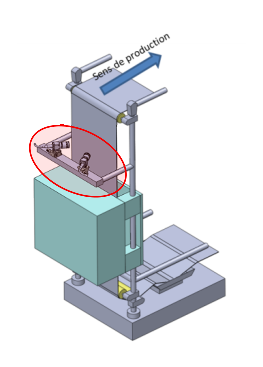
\includegraphics[width=\textwidth]{dispositif3D_bis.eps}
				\\Illustration d'un dispositif imaginé pour la caractérisation sur la machine pilote (CAO produite par Maxime \textsc{Terrien}).
			\end{center}
		\end{minipage}
	\end{frame}
	\begin{frame}{Caractérisation des défauts}
		\begin{minipage}[c]{.38\linewidth}\centering
			\includegraphics[width=\linewidth]{caracterisation_plis.pdf}
		\end{minipage}\hfill
		\begin{minipage}[c]{.57\linewidth}
			\begin{block}{Caractérisation des plis / goulottes}
				\begin{itemize}
					\item Angle par rapport au sens de production $\theta \approx \left[0, 30\right]$\si{\degres} ;
					\item Longueur $L \approx \left[10, 100\right]$\si{\centi\meter} ;
					\item Largeur $l < \SI{1}{\milli\meter}$ ;
					\item Hauteur $h < \SI{1}{\milli\meter}$) ;
					\item Répartition des défauts (nombre, orientation moyenne, fréquence d'apparition, etc.).
				\end{itemize}
			\end{block}\vspace{2em}
			\textit{Images prises par Florian \textsc{Le Gallic} (Thèse en cours).}
		\end{minipage}
	\end{frame}
	\begin{frame}{Moyen de caractérisation des défauts}
		\begin{block}{Techniques de stéréovision - méthode de dimmensionnement bien connue}
			\begin{itemize}
				\item Métrologie depuis les années 1990 : mesure des déplacements et/ou déformations d'un matériau [Faugeras (1993), Goulette (1999)].
				\item Métrologie en sollicitations dynamiques ces dernières années : augmentation de la puissance de calcul pour la corrélation temporelle et la stéréocorrélation [Abdullah (2019)].
				\item Possibilité d'obtenir des champs denses du profil altimétrique sous certaines conditions [Orteu (2002)] :
				\begin{itemize}
					\item Résolution de la caméra ;
					\item Géométrie du dispositif (angles et distances entre caméras / cible) ;
					\item Technique de mise en stéréocorrespondance (grille $\approx 1/30$ pixel ou corrélation $\approx 1/100$ pixel).
				\end{itemize}
			\end{itemize}
		\end{block}
		\begin{block}{Système de stéréovision}
			Au vu de l'encombrement des machines de production industrielles / pilote et de la contrainte de vitesse pour mener les calculs en continu, il est envisagé un système rigide à deux caméras avec vidéoprojecteur pour ajouter de la texture au matériau papier et permettre la recherche de stéréocorrespondants.
		\end{block}
	\end{frame}
	\begin{frame}{Principe de la stéréovision}
		\begin{center}
			[Graba (2005)]\\
			\includegraphics[width=.7\textwidth]{stereovision.png}
		\end{center}
		\begin{enumerate}
			\item Calibration du système optique et définition de la géométrie épipolaire ;
			\item Acquisition des images et recherche des zones stéréocorrespondantes ;
			\item Calcul de la géométrie 3D par triangulation.
		\end{enumerate}
	\end{frame}

\section{\'Etat d'avancement}
\begin{frame}{Dans cette partie...}
	\tableofcontents[sectionstyle=show/shaded, subsectionstyle=show/show/shaded]
\end{frame}

\subsection{Rappel sur l'organisation de travail}
	\begin{frame}{Tâches principales}
		En ne considérant que les aspects techniques (hors gestion du projet et valorisation des résultats), 4 tâches caractérisent l'organisation du travail :
		\begin{center}
			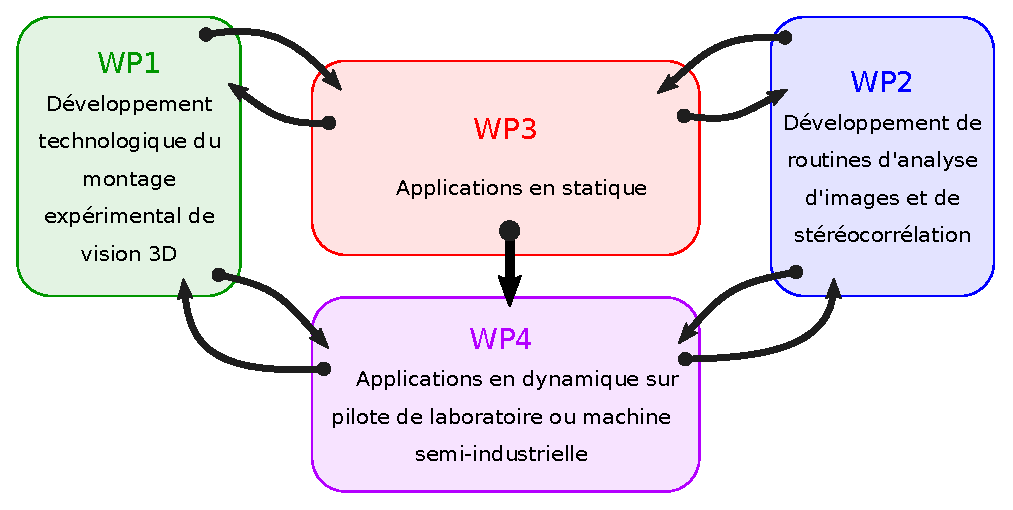
\includegraphics[width=.9\textwidth]{taches.eps}
		\end{center}
	\end{frame}

\subsection{Planning}
	\begin{frame}{Planning prévisionnel}
		\begin{center}
			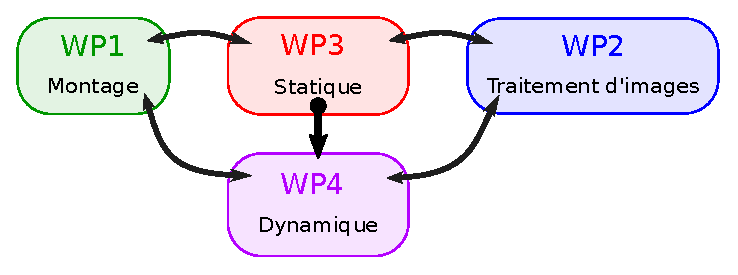
\includegraphics[width=.6\textwidth]{taches_small.eps}\vspace{2em}\\
			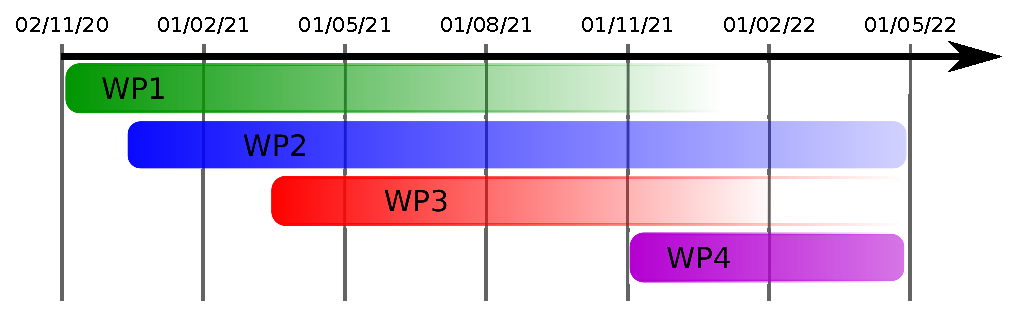
\includegraphics[width=.8\textwidth]{gant.eps}
		\end{center}
	\end{frame}
	\begin{frame}{Planning réel}
		\begin{center}
			\begin{tikzpicture}
				\draw (0, 0) node {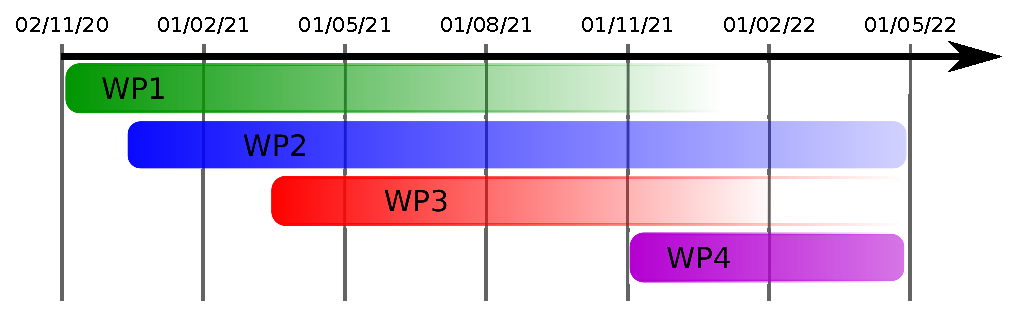
\includegraphics[width=.8\linewidth]{gant.eps}};
				\draw[densely dashed, line width=.2em] (-5.6em, -5.3em) coordinate (today) -- ++(0, 9.2em);
				\draw[stealth-] (today) -- ++(.7em, -.7em) -- ++(2em, 0) node[right] {Aujourd'hui};
			\end{tikzpicture}
		\end{center}
		\begin{exampleblock}{Planning respecté}
			Le planning est assez bien respecté. Une modification des tâches et cependant nécessaire : la calibration des systèmes optiques est intégrée dans WP2. \vspace{.5em}
			\begin{center}
			$\Rightarrow\quad$ WP2 : Développement de routines \emph{de calibration des systèmes optiques,} d’analyse d’images et de stéréocorrélation.
			\end{center}
		\end{exampleblock}
	\end{frame}


\section{Montage du dispositif en statique}
\begin{frame}{Dans cette partie...}
	\tableofcontents[sectionstyle=show/shaded, subsectionstyle=show/show/shaded]
	\begin{tikzpicture}[remember picture, overlay]
		\coordinate (C) at (current page.center);
		\draw (C) ++(3, 0) node {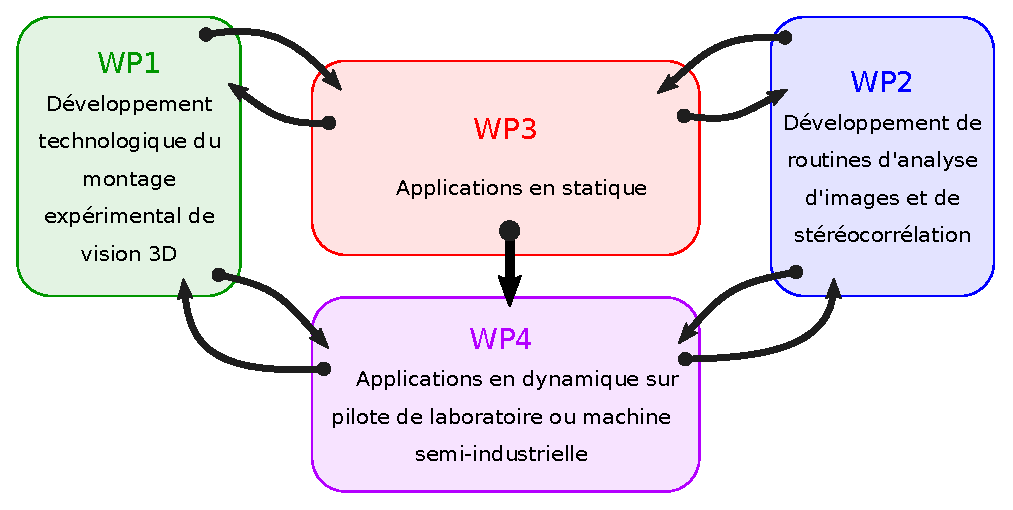
\includegraphics[width=.5\textwidth]{taches.eps}};
		\fill[white, opacity=.5] (C) ++(1.7, 1.6) rectangle ++(4.5, -3.2);
	\end{tikzpicture}
\end{frame}

\subsection{Assemblage structurel et fonctionnel}
	\begin{frame}{Dans cette partie...}
		\tableofcontents[sectionstyle=show/shaded, subsectionstyle=show/shaded/shaded]
		\begin{tikzpicture}[remember picture, overlay]
			\coordinate (C) at (current page.center);
			\draw (C) ++(3, 0) node {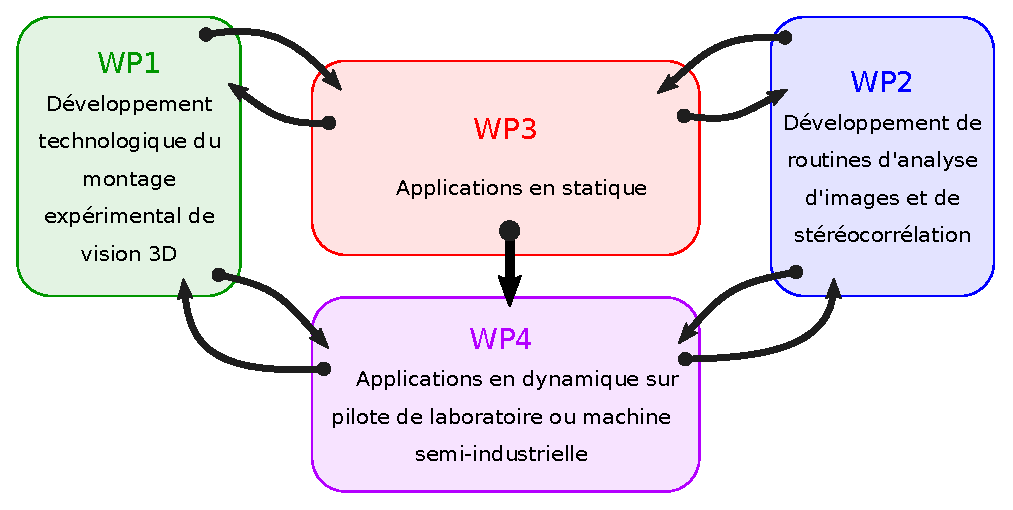
\includegraphics[width=.5\textwidth]{taches.eps}};
			\fill[white, opacity=.5] (C) ++(1.7, 1.6) rectangle ++(4.5, -3.2);
		\end{tikzpicture}
	\end{frame}
	\begin{frame}{Constitution du dispositif}
		\centering
		\begin{minipage}[c]{.38\textwidth}
			\begin{itemize}
				\item<2-> {\color[rgb]{1,0,0}Structure similaire à la machine pilote}
				\item<3-> {\color[rgb]{0,.8,0}Support des systèmes optiques}
				\item<4-> {\color[rgb]{0,0,1}Systèmes optiques}
			\end{itemize}
		\end{minipage}\hfill
		\begin{minipage}[c]{.58\textwidth}\centering
			\includegraphics[width=\textwidth]{IMG_20210222_161753_resized.jpg}
			\only<2->{
				\begin{tikzpicture}[remember picture, overlay]
				\coordinate (O) at (current page.center);
				\draw[color={rgb:red,1;green,0;blue,0}, ultra thick, opacity=.3] (O) ++ (4.22, 2.1) -- ++ (-1.3, -4.8);
				\draw[color={rgb:red,1;green,0;blue,0}, ultra thick, opacity=.3] (O) ++ (2.87, 2.47) -- ++ (-.6, -3.9);
				\end{tikzpicture}}
			\only<3->{
				\begin{tikzpicture}[remember picture, overlay]
				\coordinate (O) at (current page.center);
				\draw[color={rgb:red,.1;green,.8;blue,.1}, ultra thick, opacity=.3] (O) ++(-.31, -.7) -- ++(3.25, .3) -- ++(.69, -.93) -- ++(-4., -.85);
				\draw[color={rgb:red,.1;green,.8;blue,.1}, ultra thick, opacity=.3] (O) ++(.0, -.77) -- ++(2.3, -.52);
				\draw[color={rgb:red,.1;green,.8;blue,.1}, ultra thick, opacity=.3] (O) ++(.0, -2.35) -- ++(2.8, -.1);
				\draw[color={rgb:red,.1;green,.8;blue,.1}, ultra thick, opacity=.3] (O) ++(1.1, -1.65) -- ++(-.28, 1.3);
				\end{tikzpicture}}
			\only<4->{
				\begin{tikzpicture}[remember picture, overlay]
				\coordinate (O) at (current page.center);
				\filldraw[color={rgb:red,0;green,0;blue,1}, ultra thick, opacity=.5, fill opacity=.2] (O) ++(.5, -.28) circle (.4);
				\filldraw[color={rgb:red,0;green,0;blue,1}, ultra thick, opacity=.5, fill opacity=.2] (O) ++(.7, -1.48) circle (.5);
				\end{tikzpicture}}
		\end{minipage}
	\end{frame}
	\begin{frame}{Réglages possibles}
		\centering
		\begin{minipage}[c]{.58\textwidth}
			\begin{itemize}
				\item<2-> {\color[rgb]{1,0,0}Hauteur des systèmes optiques}
				\item<3-> {\color[rgb]{0,.8,0}Distance papier / caméras}
				\item<4-> {\color[rgb]{0,0,1}Distance entre caméra}
				\item<5-> {\color[rgb]{.56, .27, .68}Angle "de lacet" de chacune des caméras}
				\item<6-> {\color[rgb]{.95, .61, .07}Angle "de tangage" des deux caméras}
			\end{itemize}
		\end{minipage}\hfill
		\begin{minipage}[c]{.4\textwidth}\centering
			\includegraphics[width=\textwidth]{IMG_20210222_161753_resized.jpg}\\
			\includegraphics[width=\textwidth]{IMG_20210222_161728_resized.jpg}
		\end{minipage}
		\only<2->{
			\begin{tikzpicture}[remember picture, overlay]
			\coordinate (O) at (current page.center);
			\draw[color={rgb:red,1;green,0;blue,0}, ultra thick, opacity=.8, stealth-stealth] (O) ++(1.7, -2.7) -- ++(.0, -1.3);
			\draw[color={rgb:red,1;green,0;blue,0}, ultra thick, opacity=.8, stealth-stealth] (O) ++(5, -2.5) -- ++(.0, -1.5);
			\end{tikzpicture}}
		\only<3->{
			\begin{tikzpicture}[remember picture, overlay]
			\coordinate (O) at (current page.center);
			\draw[color={rgb:red,0.1;green,0.8;blue,0.1}, ultra thick, opacity=.8, stealth-stealth] (O) ++(2., .9) -- ++(1.7, .25);
			\end{tikzpicture}}
		\only<4->{
			\begin{tikzpicture}[remember picture, overlay]
			\coordinate (O) at (current page.center);
			\draw[color={rgb:red,0;green,0;blue,1}, ultra thick, opacity=.8, stealth-stealth] (O) ++(2.8, -1.6) -- ++(1.1, .0);
			\end{tikzpicture}}
		\only<5->{
			\begin{tikzpicture}[remember picture, overlay]
			\coordinate (O) at (current page.center);
			\draw[color={rgb:red,.82;green,.39;blue,1}, ultra thick, opacity=.8, <->] (O) ++(2.7, -1.) arc (40:320:.7cm and .1cm);
			\draw[color={rgb:red,.82;green,.39;blue,1}, ultra thick, opacity=.8, <->] (O) ++(3.8, -1.) arc (140:-140:.7cm and .1cm);
			\end{tikzpicture}}
		\only<6->{
			\begin{tikzpicture}[remember picture, overlay]
			\coordinate (O) at (current page.center);
			\draw[color={rgb:red,1;green,.64;blue,.07}, ultra thick, opacity=.8, <->] (O) ++(2.6, .4) arc (30:350:.2cm and .27cm);
			\end{tikzpicture}}
	\end{frame}

\subsection{Systèmes optiques}
	\begin{frame}{Dans cette partie...}
		\tableofcontents[sectionstyle=show/shaded, subsectionstyle=show/shaded/shaded]
		\begin{tikzpicture}[remember picture, overlay]
			\coordinate (C) at (current page.center);
			\draw (C) ++(3, 0) node {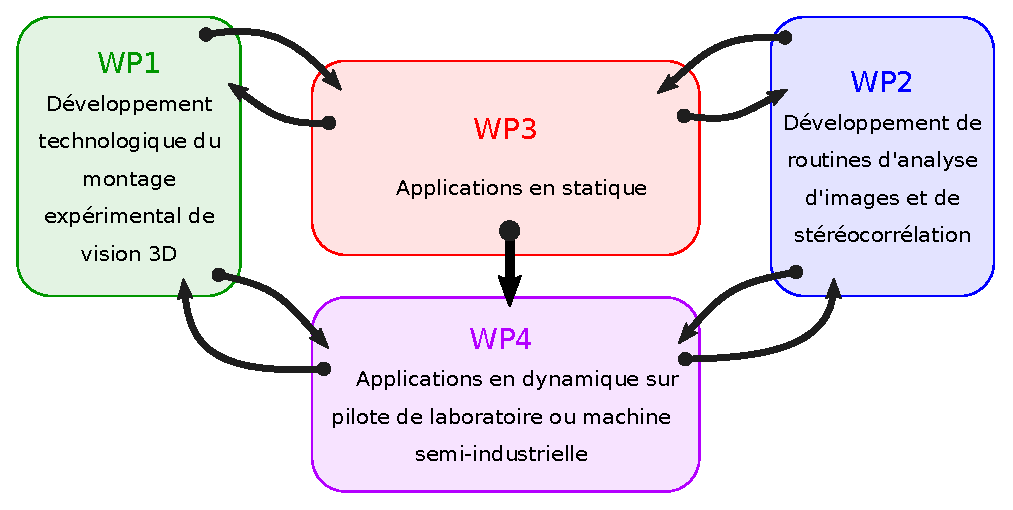
\includegraphics[width=.5\textwidth]{taches.eps}};
			\fill[white, opacity=.5] (C) ++(1.7, 1.6) rectangle ++(4.5, -3.2);
		\end{tikzpicture}
	\end{frame}
	\begin{frame}{Appareil photographique numérique (APN)}
		\begin{block}{Propriétés du capteur associé au Canon EOS 1200D}\centering
			\begin{tabular}{>{\bfseries}r@{\hspace{1em}}l}
				\hline
				Format & APS-C (\SI{22.3 x 14.9}{\milli\meter})\\
				Pixels effectifs & \num{18}~MPx \\
				Ratio de format & 3: 2 \\
				Filtre passe bas & intégré\\
				\hline\vspace{.5em}
			\end{tabular}
		\end{block}
		\begin{center}
			\includegraphics[width=.7\linewidth]{canonEOS1200D.jpg}
		\end{center}
	\end{frame}
	\begin{frame}{Objectif à focale fixe adaptable à l'APN}
		\begin{block}{Propriétés de l'objectif Canon EF-S 24~mm f/2.8 STM}\centering
			\begin{tabular}{>{\bfseries}r@{\hspace{1em}}l}
				\hline
				Focale équivalente (\SI{36 x 24}{\milli\meter}) & \SI{38}{\milli\meter}\\
				Distance minimale mise au point & \SI{160}{\milli\meter}\\
				Autofocus motorisé & oui\\
				Angle de champ horizontal & \ang{59;10;}\\
				Angle de champ vertical & \ang{50;35;}\\
				\hline\vspace{.05em}
			\end{tabular}
		\end{block}
		\begin{center}
			\includegraphics[width=.7\linewidth]{canonEFS24mm.jpg}
		\end{center}
	\end{frame}
	\begin{frame}{Utilisation des systèmes optiques}
		\begin{block}{Résolution}
			Dans ce projet, les APN auront un champ de vision horizontal d'environ \SI{35}{\centi\meter}. Les images obtenues présentent l'axe horizontal selon approximativement \SI{5000}{pixels}.
			\begin{center}$\Rightarrow\quad$ Taille du pixel : $\approx \SI{70}{\micro\meter}$\end{center}
		\end{block}
		\begin{block}{Méthode d'utilisation}
			\begin{itemize}
				\item 1 APN = 1 objectif : pas de changement grâce à l'étiquetage
				\item Calibration de l'ensemble (APN + objectif) si changement
				\item Calibration du système stéréoscopique après chaque changement de réglage du montage
				\item Prise de vue du sujet et enregistrement sur carte SD au format JPG (18~ MPx)
				\item Post-traitement sur ordinateur. Mise en veille de l'expérimentation et protection des équipements
			\end{itemize}
		\end{block}
	\end{frame}


\section{Travaux numériques}
\begin{frame}{Dans cette partie...}
	\tableofcontents[sectionstyle=show/shaded, subsectionstyle=show/show/shaded]
	\begin{tikzpicture}[remember picture, overlay]
		\coordinate (C) at (current page.center);
		\draw (C) ++(3, 0) node {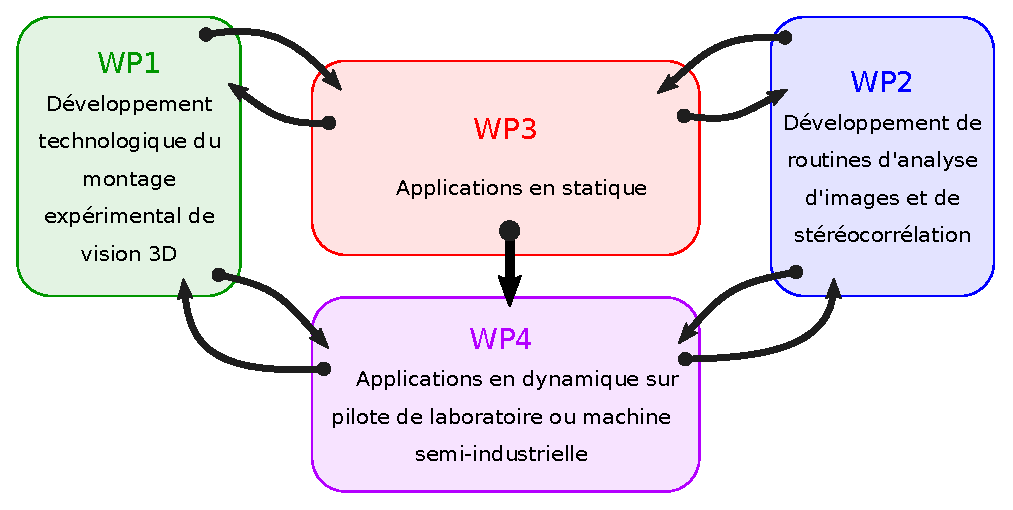
\includegraphics[width=.5\textwidth]{taches.eps}};
		\fill[white, opacity=.5] (C) ++(-.1, 1.6) rectangle ++(1.7, -3.2);
		\fill[white, opacity=.5] (C) ++(1.6, -1.6) rectangle ++(3, 1.5);
	\end{tikzpicture}
\end{frame}

\subsection{Librairie Python ds3dlive}
	\begin{frame}{Dans cette partie...}
		\tableofcontents[sectionstyle=show/shaded, subsectionstyle=show/shaded/shaded]
		\begin{tikzpicture}[remember picture, overlay]
			\coordinate (C) at (current page.center);
			\draw (C) ++(3, 0) node {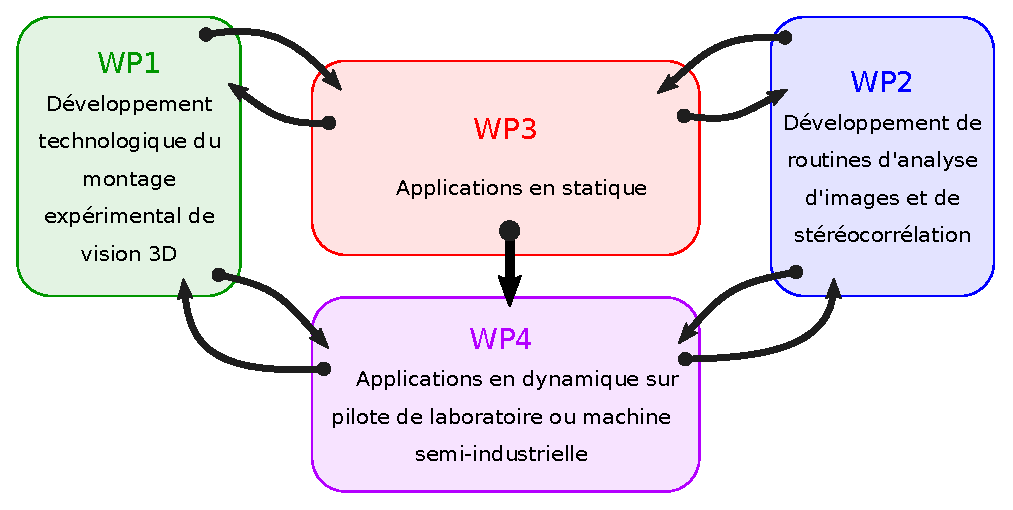
\includegraphics[width=.5\textwidth]{taches.eps}};
			\fill[white, opacity=.5] (C) ++(-.1, 1.6) rectangle ++(1.7, -3.2);
			\fill[white, opacity=.5] (C) ++(1.6, -1.6) rectangle ++(3, 1.5);
		\end{tikzpicture}
	\end{frame}
	\begin{frame}{Quelques règles d'un travail bien fait en développement numérique}
		Afin d'assurer une bonne distribution, une utilisation facile pour l'utilisateur et une longue durée de vie à un programme, il est nécessaire de respecter les règles qui suivent :
		\vspace{1em}
		\begin{itemize}[<+->]
			\item Fonctionnaliser les tâches ;
			\item Donner de la modularité aux algorithmes ;
			\item User des avantages de la programmation orientée objet ;
			\item Rendre distribuables les librairies, dans la mesure du possible ;
			\item Tester l'ensemble des modules ;
			\item Utiliser des programmes de versionnage qui enregistre toutes les modifications et permettent de retrouver un état antérieur et de collaborer avec d'autres développeurs.
		\end{itemize}
	\end{frame}
	\begin{frame}{Pour le projet DS3DLive}
		\begin{itemize}
			\item Création d'une librairie "ds3dlive" ;
			\item Création de modules (calibration, simulation, stereo, wrinkle, ...) ;
			\item Création d'objets adéquats (Camera, Stereosystem, WrinkleDetector, ...) ;
			\item Projet ouvert sur GitHub (en privé) ;
			\item Tests unitaires sur l'ensemble des fonctions ;
			\item Versionnage par l'intermédiaire de Git en utilisant un modèle GitFlow.
		\end{itemize}
	\end{frame}
	\begin{frame}{Consitution de la librairie}
		\begin{center}
			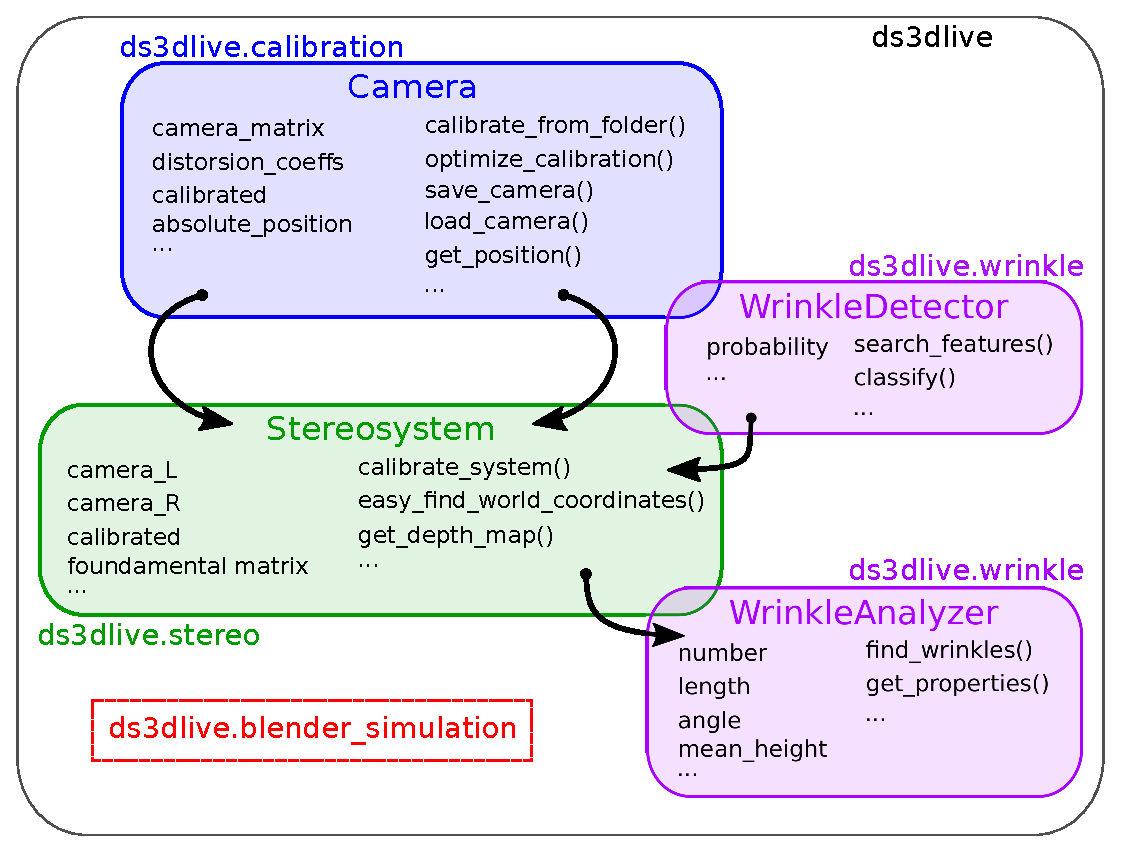
\includegraphics[width=.8\linewidth]{logigramme.eps}
		\end{center}
	\end{frame}

\subsection{Calibration des systèmes optiques}
	\begin{frame}{Dans cette partie...}
		\tableofcontents[sectionstyle=show/shaded, subsectionstyle=show/shaded/shaded]
		\begin{tikzpicture}[remember picture, overlay]
			\coordinate (C) at (current page.center);
			\draw (C) ++(0, 2.5) coordinate (T);
			\draw (C) ++(0, -1.5) coordinate (B);
			\draw (T) ++(3, 0) node {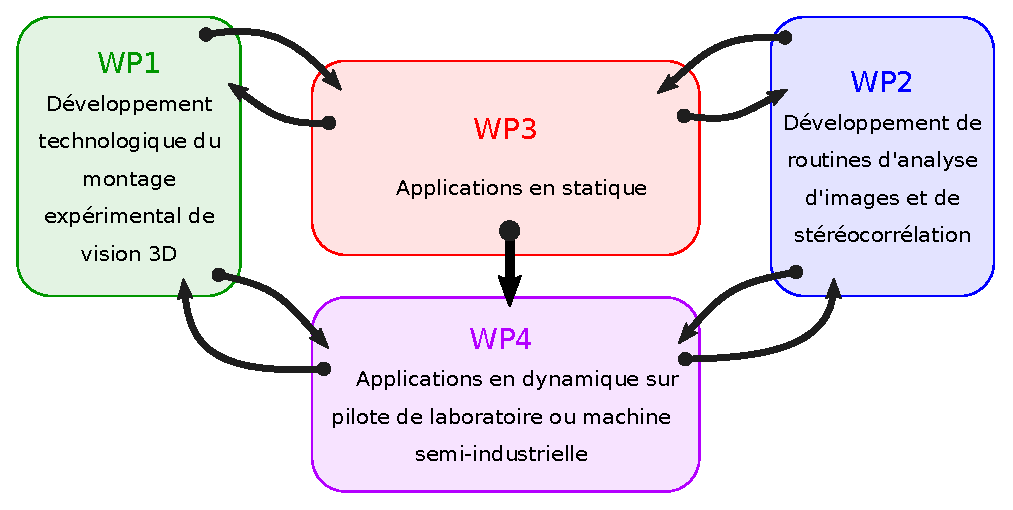
\includegraphics[width=.5\textwidth]{taches.eps}};
			\fill[white, opacity=.5] (T) ++(-.1, 1.6) rectangle ++(1.7, -3.2);
			\fill[white, opacity=.5] (T) ++(1.6, -1.6) rectangle ++(3, 1.5);
			\draw (B) ++(3, 0) node {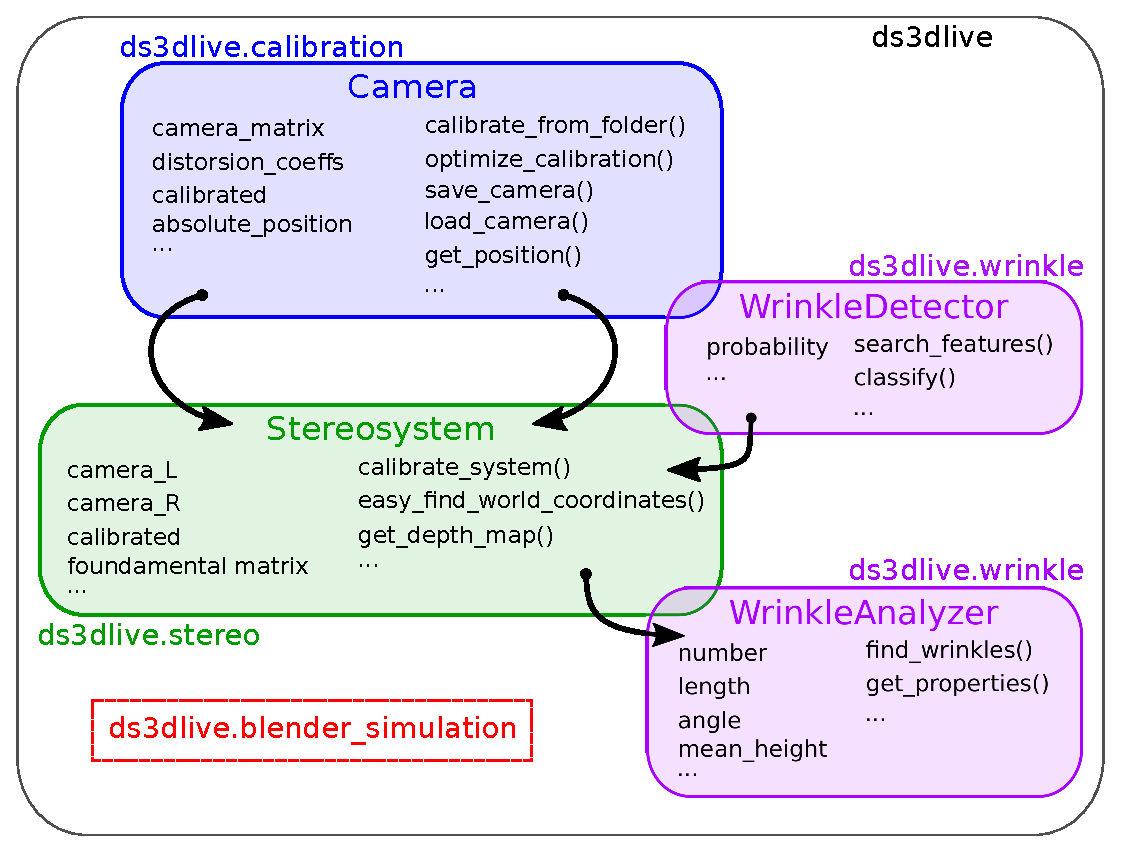
\includegraphics[width=.5\textwidth]{logigramme.eps}};
			\fill[white, opacity=.5] (B) ++(0, .6) rectangle ++(4, -1.9);
			\fill[white, opacity=.5] (B) ++(4, 1.5) rectangle ++(1.95, -3.6);
			\fill[white, opacity=.5] (B) ++(.3, -1.3) rectangle ++(3.7, -.85);
		\end{tikzpicture}
	\end{frame}
	\begin{frame}{Méthode par la correspondance points 3D - points image}
		\begin{block}{Mire de calibration}
			Une mire de calibration est nécessaire. Il s'agit d'un support physique sur lequel sont placés des éléments faciles à segmenter à des positions très précises. La réalisation d'une telle mire permet de déterminer une liste de points 3D (un point par élément à segmenter).
			\begin{center}
				\includegraphics[width=.28\textwidth, angle=90]{chessBoard14x10_25mm.pdf}
			\end{center}
		\end{block}
		\begin{block}{Mise en correspondance}
			La segmentation des images de la mire permet de générer une liste de points images, associés aux points 3D (il est donc important de les ranger dans le même ordre).
			\\La librairie OpenCV est utilisée ici car elle possède un module de calibration 3D.
		\end{block}
	\end{frame}
	\begin{frame}{Résolution par la minimisation des moindres carrés}
		\begin{block}{On cherche à résoudre pour les $n$ points correspondants}
			$$\forall p = 1, \cdots, n \qquad
			q_p = \begin{pmatrix}
			u_p\\v_p\\1
			\end{pmatrix} \sim P \begin{pmatrix}
			X_p\\Y_p\\Z_p
			\end{pmatrix} \sim PQ_p \quad \Rightarrow \quad
			\begin{pmatrix}
			u_p\\v_p
			\end{pmatrix} = \begin{pmatrix}
			(PQ_p)_1 / (PQ_p)_3\\(PQ_p)_2 / (PQ_p)_3
			\end{pmatrix}
			$$
			Les équations sont linéaires en les éléments de $P$ et les composantes de $P$ peuvent donc être retrouvées.
		\end{block}
		\begin{block}{Minimisation par les moindre carrés}
			\`A cause du bruit dans les images et des erreurs typiques des expérimentations, il serait plus que hasardeux de tomber sur l'unique solution à partir d'un minimum de 12 points. L'ensemble des points sont alors utilisés et on cherche finalement à résoudre l'équation par une méthode des moindres carrés.
		\end{block}
		\begin{block}{Recherche de $K$, $R$ et $t$ à partir de $P$}
			Connaissant les composantes de $P$ il est possible de définir les composantes de $K$ (donc les paramètres intrinsèques, ce qui est souvent recherché) mais aussi les paramètres extrinsèques. 
		\end{block}
	\end{frame}
	\begin{frame}{\'Edition automatique d'une mire de type damier}
		\begin{block}{Script \LaTeX}
			Un script a été écrit pour être compilé en \LaTeX. Il y a trois paramètres :
			\begin{itemize}
				\item Taille des carrés en millimètre ;
				\item Nombre de lignes souhaitées ;
				\item Nombre de colonnes souhaitées.
			\end{itemize}
			La sortie est un fichier PDF (donc image vectorielle) contenant uniquement le damier (aucun espace inutile). Une impression en taille réelle permet d'obtenir une mire très précise.
		\end{block}
		\begin{exampleblock}{Exemple}\centering
			\includegraphics[height=.3\textwidth, angle=90]{chessBoard14x10_25mm.pdf}
			\hfill
			\includegraphics[height=.3\textwidth, angle=90]{chessBoard16x10_20mm.pdf}
			\hfill
			\includegraphics[height=.3\textwidth, angle=90]{chessBoard22x14_15mm.pdf}\\
			\SI{25}{\milli\meter} $14 \times 10$\hfill
			\SI{20}{\milli\meter} $16 \times 10$\hfill
			\SI{15}{\milli\meter} $22 \times 14$
		\end{exampleblock}
	\end{frame}
	\begin{frame}{Prise d'images avec mire}\centering
		\begin{block}{Règle}
			Prendre plusieurs images (plus d'une douzaine) avec différents angles et permettant d'observer l'intégralité de la mire.
		\end{block}
		\begin{exampleblock}{Exemple}
			\begin{minipage}[t]{.48\textwidth}\centering
				Caméra Gauche
			\end{minipage}\hfill
			\begin{minipage}[t]{.48\textwidth}\centering
				Caméra Droite
			\end{minipage}\vspace{1em}\\
			\begin{minipage}[c]{.48\textwidth}\centering
				\animategraphics[autoplay, loop, width=\textwidth]{3}{left_camera/small_IMG_}{8839}{8866}
			\end{minipage}\hfill
			\begin{minipage}[c]{.48\textwidth}\centering
				\animategraphics[autoplay, loop, width=\textwidth]{3}{right_camera/small_IMG_}{8855}{8883}
			\end{minipage}
		\end{exampleblock}
	\end{frame}
	\begin{frame}{Illustration de l'effet de la distorsion}\centering
		\begin{block}{Caméra Droite}
			\begin{itemize}
				\item Matrice de caméra :
				$$\begin{pmatrix}
				\num{5.93083e+03} & 0 & \num{2.50473e+03} \\
				0 & \num{5.94430e+03} & \num{1.76974e+03} \\
				0 & 0 & 1
				\end{pmatrix}$$
				\item Coefficients de distorsion :
				$$\left(
				\num{-1.47e-1}, \num{8.82e-1}, \num{1.42e-3}, \num{-2.39e-3}, \num{-3.59}
				\right)$$
			\end{itemize}
		\end{block}
		\begin{minipage}[c]{.45\textwidth}
			\includegraphics[width=\textwidth]{distorted_resized.jpg}
		\end{minipage}\hfill
		\begin{minipage}[c]{.08\textwidth}\centering
			$\longrightarrow$
		\end{minipage}\hfill
		\begin{minipage}[c]{.45\textwidth}
			\includegraphics[width=\textwidth]{regletR_undistorted_small.jpg}
		\end{minipage}
	\end{frame}

\subsection{Système stéréoscopique}
	\begin{frame}{Dans cette partie...}
		\tableofcontents[sectionstyle=show/shaded, subsectionstyle=show/shaded/shaded]
		\begin{tikzpicture}[remember picture, overlay]
			\coordinate (C) at (current page.center);
			\draw (C) ++(0, 2.5) coordinate (T);
			\draw (C) ++(0, -1.5) coordinate (B);
			\draw (T) ++(3, 0) node {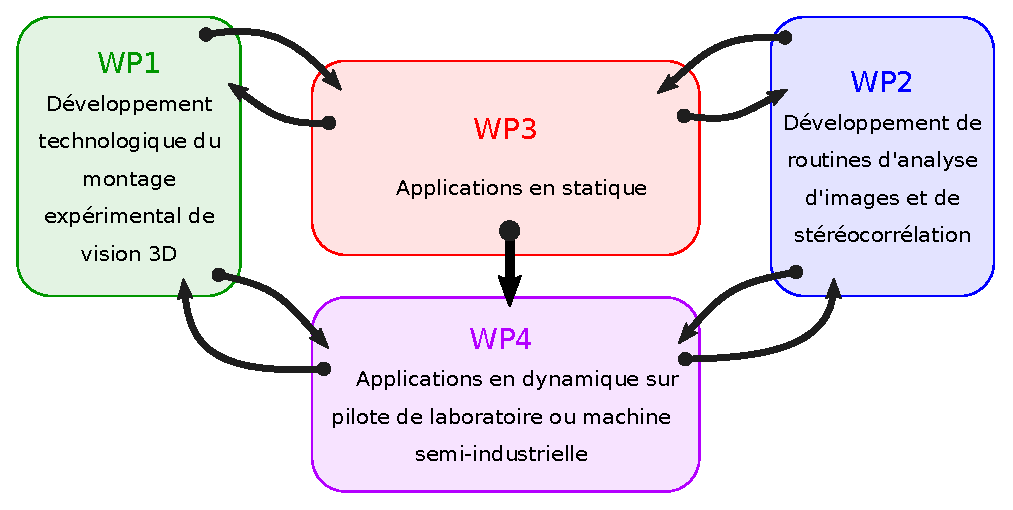
\includegraphics[width=.5\textwidth]{taches.eps}};
			\fill[white, opacity=.5] (T) ++(-.1, 1.6) rectangle ++(1.7, -3.2);
			\fill[white, opacity=.5] (T) ++(1.6, -1.6) rectangle ++(3, 1.5);
			\draw (B) ++(3, 0) node {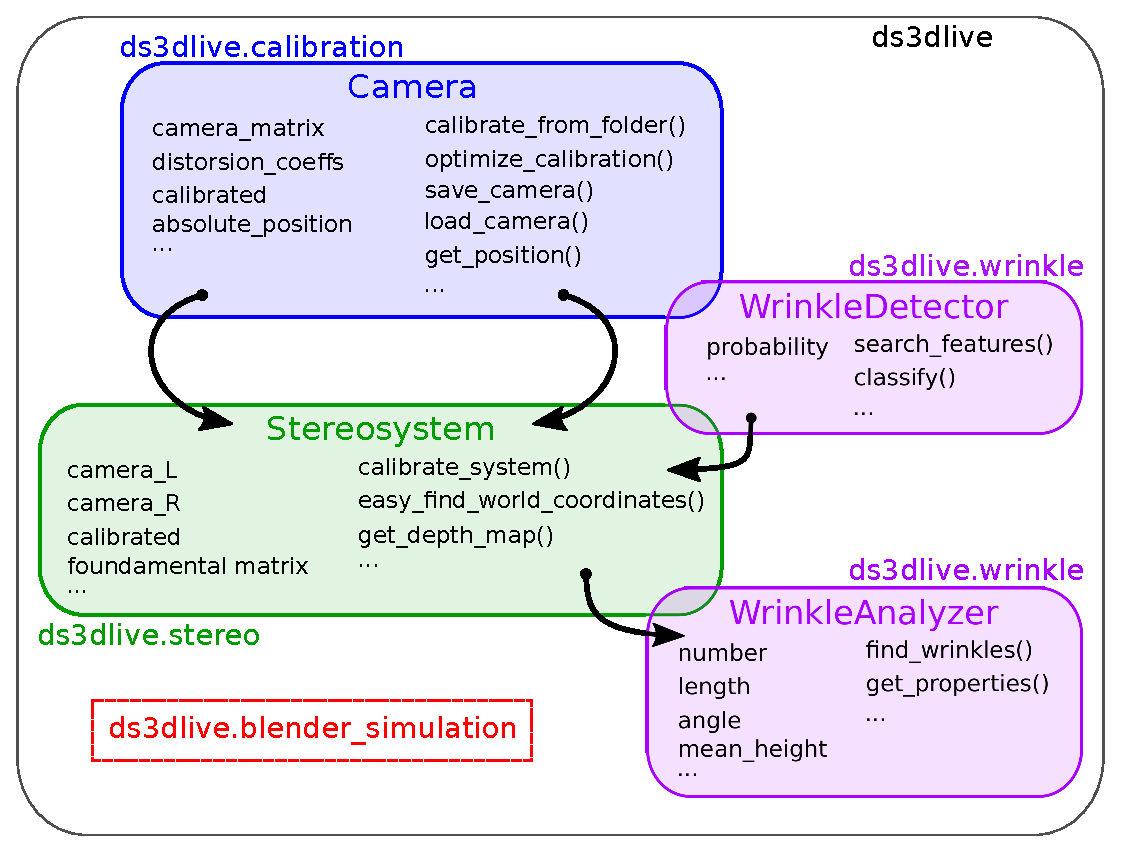
\includegraphics[width=.5\textwidth]{logigramme.eps}};
			\fill[white, opacity=.5] (B) ++(.35, 0.15) rectangle ++(3.6, 2.1);
			\fill[white, opacity=.5] (B) ++(3.95, 1.5) rectangle ++(2, -3.6);
			\fill[white, opacity=.5] (B) ++(.3, -1.3) rectangle ++(3.65, -.85);
			\fill[white, opacity=.5] (B) ++(1.5, -1.3) rectangle ++(2.45, .2);
		\end{tikzpicture}
	\end{frame}
	\begin{frame}{Contrainte épipolaire pour la recherche des stéréocorrespondants}
		\begin{block}{Contrainte épipolaire - Matrice fondamentale}
			Considérant deux points stéréocorrespondants, $q_1$ et $q_2$, la géométrie épipolaire établie une contrainte qui stipule qu'il est possible de trouver, à partir d'un des points stéréocorrespondants, l'autre point en cherchant le long d'une droite.
			\\Mathématiquement, on introduit la matrice fondamentale $F$ de taille \num{3x3} pour décrire cette contrainte :
			$$
			q_2^T \cdot F \cdot q_1 = 0
			$$
		\end{block}
		\begin{block}{Contrainte épipolaire calibrée - Matrice essentielle}
			Contrainte épipolaire en considérant les repères images. On définit maintenant la matrice essentielle $E$ qui correspond à la matrice fondamentale exprimée en longueur métrique (non plus en pixels) :
			$$
			E \sim {K_2}^T \cdot F \cdot K_1
			$$
		\end{block}
		\begin{block}{Calibration du système stéréoscopique}
			Dans le cadre de ce projet, le système stéréoscopique n'est pas voué à changer de position trop souvent. Il y a alors un fort intérêt à calibrer le système en calculant précisément les positions de chacune des caméras. On peut ainsi déterminer directement la matrice essentielle $E$ grâce aux paramètres extrinsèques.
		\end{block}
	\end{frame}
	\begin{frame}{Reconstruction 3D}
		\begin{block}{Globalement, en connaissant les paramètres intrinsèques et extrinsèques}
			Il est possible de déterminer les coordonnées d'un point $Q$ dans l'espace à partir de la connaissance des ces coordonnées $q_i$ dans $i$ images :
			$$
			\forall i,\qquad P_iQ \sim q_i
			$$
		\end{block}
		\begin{block}{Si l'on ne connait pas les paramètres extrinsèques}
			\begin{itemize}
				\item On détermine la pose d'un objet pour chaque caméra (il s'agit de retrouver la position de la caméra par rapport à l'objet)
				\item On considère la contrainte épipolaire pour rechercher des points stéréocorrespondants et outrepasser la connaissance des paramètres extrinsèques
			\end{itemize}
		\end{block}\vspace{1em}
		\begin{center}
			Démonstration en direct !
		\end{center}
	\end{frame}

\subsection{Simulation 3D}
	\begin{frame}{Dans cette partie...}
		\tableofcontents[sectionstyle=show/shaded, subsectionstyle=show/shaded/shaded]
		\begin{tikzpicture}[remember picture, overlay]
			\coordinate (C) at (current page.center);
			\draw (C) ++(0, 2.5) coordinate (T);
			\draw (C) ++(0, -1.5) coordinate (B);
			\draw (T) ++(3, 0) node {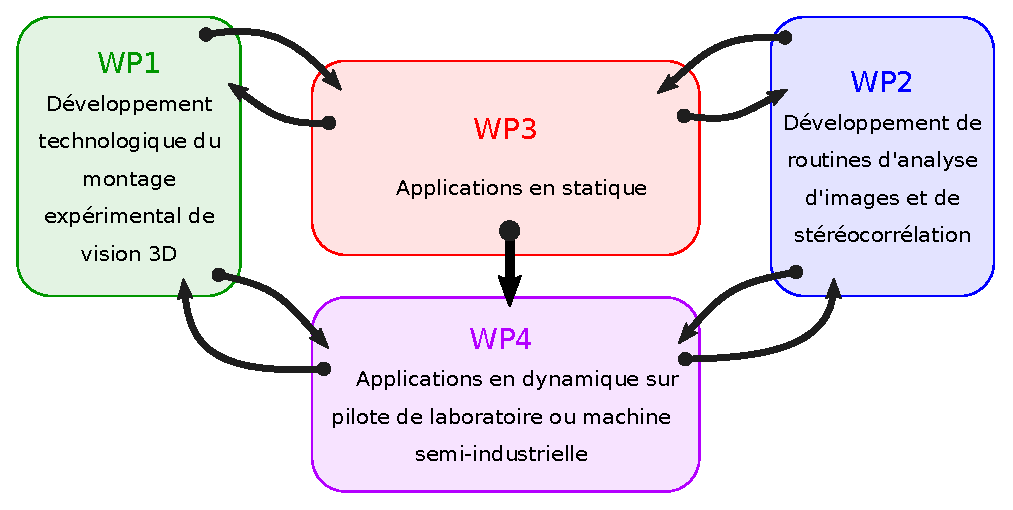
\includegraphics[width=.5\textwidth]{taches.eps}};
			\fill[white, opacity=.5] (T) ++(-.1, 1.6) rectangle ++(1.7, -3.2);
			\fill[white, opacity=.5] (T) ++(1.6, -1.6) rectangle ++(3, 1.5);
			\draw (B) ++(3, 0) node {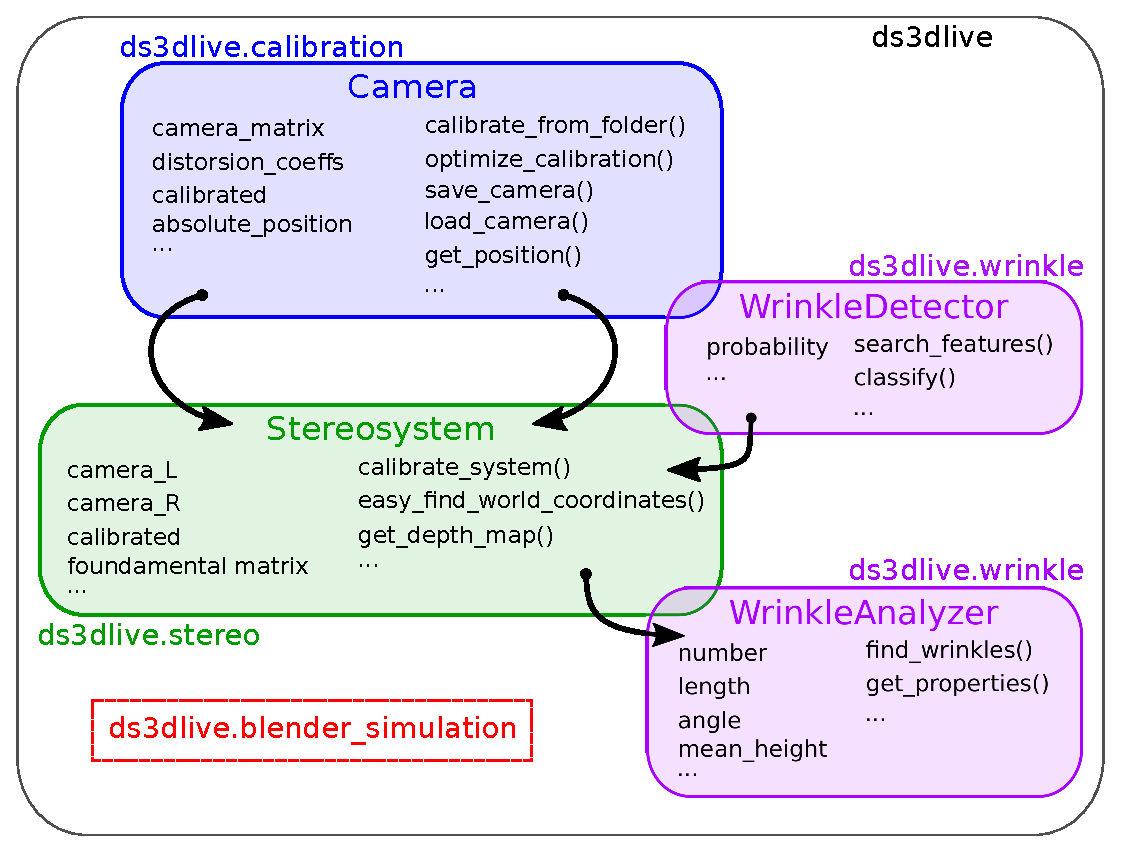
\includegraphics[width=.5\textwidth]{logigramme.eps}};
			\fill[white, opacity=.5] (B) ++(.35, 0.15) rectangle ++(3.6, 2.1);
			\fill[white, opacity=.5] (B) ++(3.95, 1.5) rectangle ++(2, -3.6);
			\fill[white, opacity=.5] (B) ++(0, -1.3) rectangle ++(3.95, 1.45);
			\fill[white, opacity=.5] (B) ++(3.2, -1.3) rectangle ++(.75, -.8);
		\end{tikzpicture}
	\end{frame}
	\begin{frame}
		\frametitle{Utilisation de Blender}
		\begin{minipage}[c]{.35\textwidth}
			\begin{block}{\'Etapes de réalisation de la simulation}
				\setbeamercovered{transparent}
				\begin{enumerate}
					\item<1-> Création du projet Blender
					\item<2-> Ajout de la première caméra
					\item<3-> Ajout de la seconde caméra
					\item<4-> Ajout du papier avec pli vertical
					\item<5-> Ajout d'un "monde" réaliste\footnotemark
					\item<6-> Acquisition des images de rendu
				\end{enumerate}
			\end{block}
		\end{minipage}\hfill
		\begin{minipage}[c]{.6\textwidth}\centering
			\only<1>{
				\begin{figure}
					\includegraphics[width=\textwidth]{screen_0_resized.png}
					\caption{Création du projet Blender}
			\end{figure}}
			\only<2>{
				\begin{figure}
					\includegraphics[width=\textwidth]{screen_1_resized.png}
					\caption{Ajout de la première caméra}
			\end{figure}}
			\only<3>{
				\begin{figure}
					\includegraphics[width=\textwidth]{screen_2_resized.png}
					\caption{Ajout de la seconde caméra}
			\end{figure}}
			\only<4>{
				\begin{figure}
					\includegraphics[width=\textwidth]{screen_3_resized.png}
					\caption{Ajout du papier avec pli vertical}
			\end{figure}}
			\only<5>{
				\begin{figure}
					\includegraphics[width=\textwidth]{screen_4_resized.png}
					\caption{Ajout d'un "monde" réaliste}
			\end{figure}}
			\only<6>{
				\begin{figure}
					\includegraphics[width=.85\textwidth]{view_0_resized.jpg}\\
					\includegraphics[width=.85\textwidth]{view_1_resized.jpg}
					\caption{Acquisition des images de rendu}
			\end{figure}}
		\end{minipage}
		\uncover<5>{\footnotetext{Dont ajout d'un éclairage apporté, qui n'est pas illustré ici.}}
	\end{frame}
	\begin{frame}
		\frametitle{Automatisation de la simulation à partir d'un fichier de paramètres}
		\begin{block}{Utilisation d'un script Python pour l'automatisation des tâches}
			L'interface de Blender étant essentiellement développée en Python, il est possible d'écrire un script Python qui interagit avec le logiciel. Il est nécessaire pour cela d'utiliser les outils de l'API (Application Programming Interface) de Blender.
		\end{block}
		\begin{block}{Création d'un module pour le projet}
			Un module permettant l'importation de fonctions et classes appropriées au projet a été créé. Ce module peut être réutilisable pour d'autres simulations du même type.
		\end{block}
		\begin{block}{Simulations paramétriques et classification des résultats}
			Grâce à la modularité du programme, il est possible de mener des campagnes de simulation en faisant varier les paramètres à notre guise. Par exemple, il est possible de mener, de manière automatique, des simulations pour différents angles des caméras avec des pas de \ang{.5}.
			\\Les résultats (exemple: les images acquises par les caméras), sont enregistrés dans un dossier avec un fichier rappelant les paramètres utilisés. Un dictionnaire parent est également présent pour retrouvé facilement une simulation à partir de fonctions de tri / filtres.
		\end{block}
	\end{frame}
	\begin{frame}
		\frametitle{Paramètres à considérés}
		\begin{block}{Paramètres propre au dispositif}
			\begin{multicols}{3}
				\begin{itemize}
					\item Distance caméra 1 / caméra 2
					\item Distance caméras / papier
					\item Angles des caméras
					\item Largeur du papier
					\item Largeur, position et résolution du pli
					\item Longueurs focales des caméras
					\item \'Eclairages
					\item Autres à venir...
				\end{itemize}
			\end{multicols}
		\end{block}
		\begin{block}{Paramètres physiques - Méthode procédurale pour créer le matériau "papier"}
			\begin{multicols}{2}
				\begin{itemize}
					\item Texture prédéfinie (pas obligatoire)
					\item Rugosité
					\item Autres à venir...
					\item Effet "subsurface" (transmission partielle de l'éclairage sur l'épaisseur du matériau avec potentielle modification des couleurs)
				\end{itemize}
			\end{multicols}
		\end{block}
		\begin{block}{Paramètres de rendu des images}
			\begin{multicols}{3}
				\begin{itemize}
					\item Moteur de rendu
					\item Insertion du monde dans la scène
					\item Type et méthodes de calcul
					\item Taille et format des images de sortie
					\item Nombre d'images moyennées
					\item Gestion des sauvegardes
					\item Autres à venir...
				\end{itemize}
			\end{multicols}
		\end{block}
	\end{frame}

\subsection{Caractérisation des plis}
	\begin{frame}{Dans cette partie...}
		\tableofcontents[sectionstyle=show/shaded, subsectionstyle=show/shaded/shaded]
		\begin{tikzpicture}[remember picture, overlay]
			\coordinate (C) at (current page.center);
			\draw (C) ++(0, 2.5) coordinate (T);
			\draw (C) ++(0, -1.5) coordinate (B);
			\draw (T) ++(3, 0) node {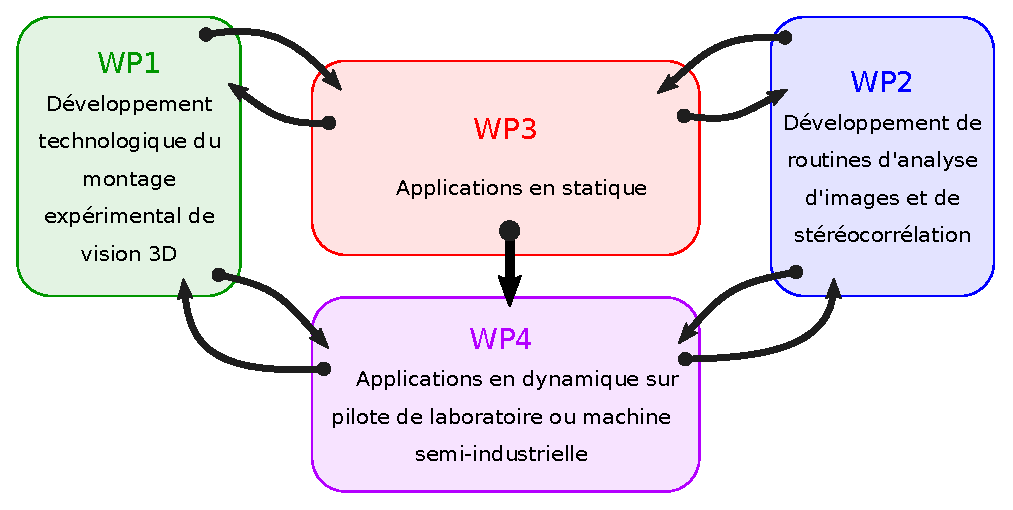
\includegraphics[width=.5\textwidth]{taches.eps}};
			\fill[white, opacity=.5] (T) ++(-.1, 1.6) rectangle ++(1.7, -3.2);
			\fill[white, opacity=.5] (T) ++(1.6, -1.6) rectangle ++(3, 1.5);
			\draw (B) ++(3, 0) node {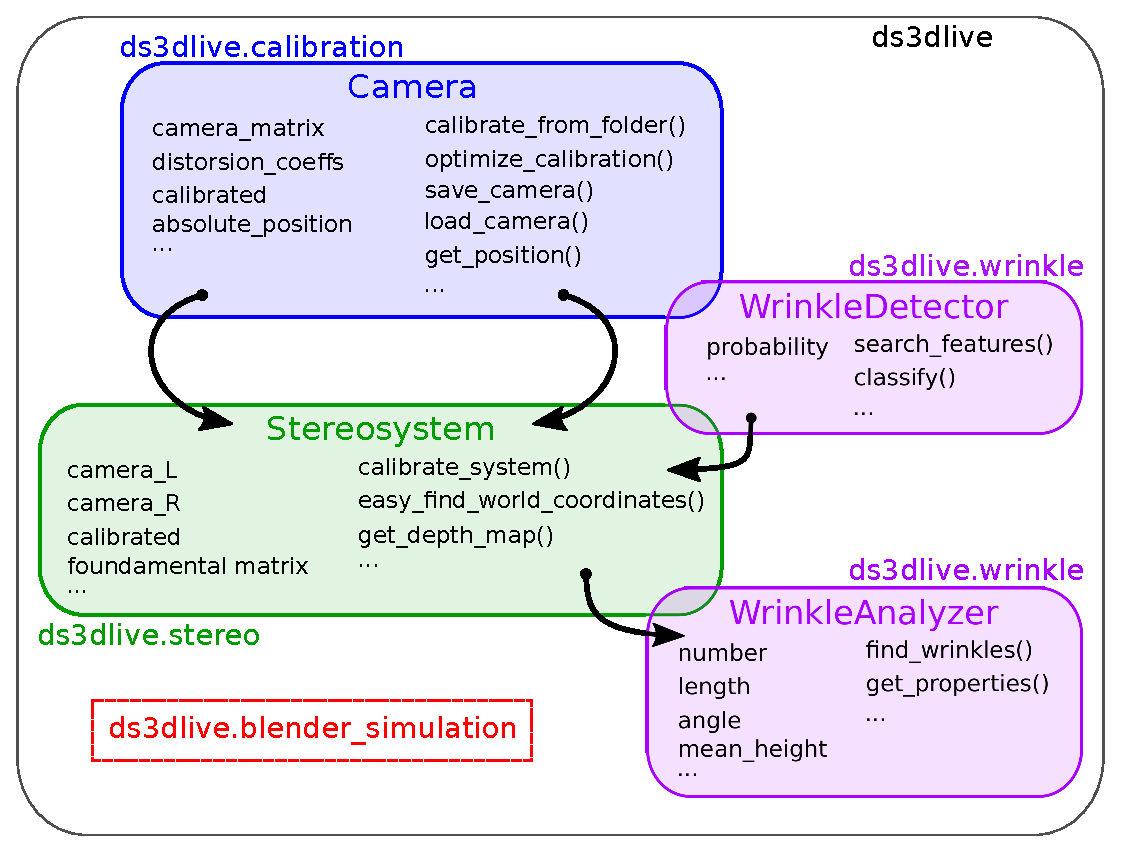
\includegraphics[width=.5\textwidth]{logigramme.eps}};
			\fill[white, opacity=.5] (B) ++(.35, 0.15) rectangle ++(3.6, 2.1);
			\fill[white, opacity=.5] (B) ++(3.95, 1.5) rectangle ++(2, -2);
			\fill[white, opacity=.5] (B) ++(0, -.85) rectangle ++(3.95, 1.0);
			\fill[white, opacity=.5] (B) ++(0, -.85) rectangle ++(3.4, -1.1);
		\end{tikzpicture}
	\end{frame}
	\begin{frame}{Caractérisation géométrique d'un pli}
		\begin{block}{Ordre de grandeur des défauts}
			Une première caractérisation d'un pli a été mené sur Alicona Infinite Focus afin de déterminer un ordre de grandeur des dimensions d'un pli type. Dix-huit points de mesures ont été analysés sur une longueur de \SI{35}{\milli\meter}. La hauteur du pli est en moyenne de \SI{707(74)}{\micro\meter} et son épaisseur à mi-hauteur de \SI{680(167)}{\micro\meter}. Une résolution permettant d'avoir une précision en $Z$ de l'ordre de \SI{50}{\micro\meter} semble bien adaptée.
		\end{block}
		\begin{minipage}[c]{0.49\textwidth}
			\begin{figure}\centering
				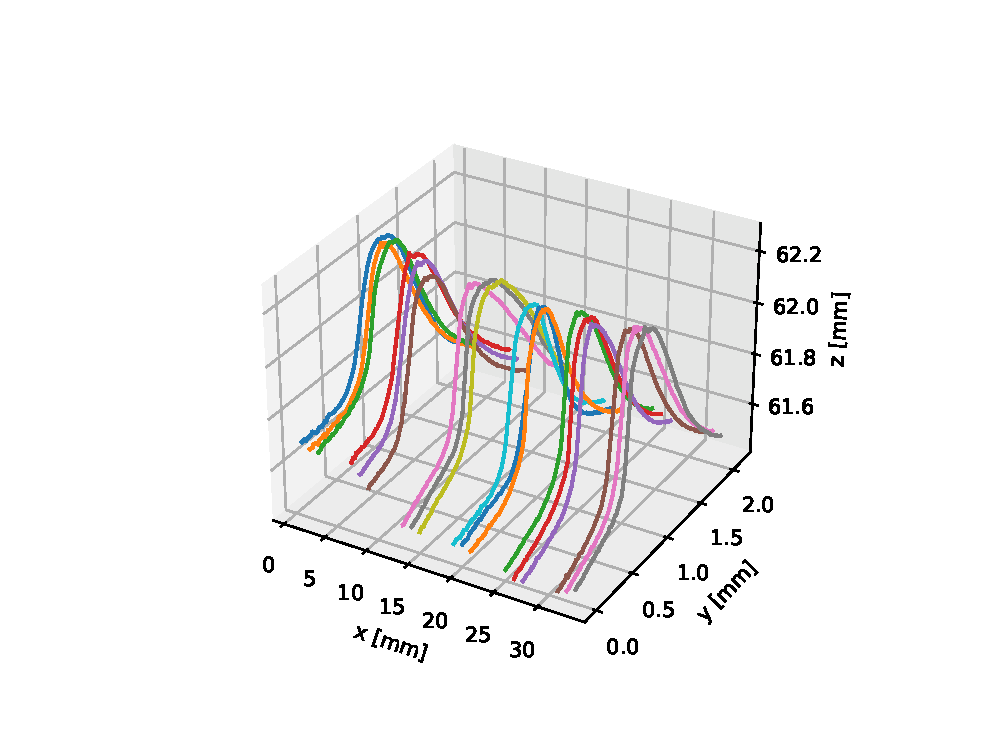
\includegraphics[width=1.\textwidth]{profiles.eps}
				\caption{Profils linéiques d'un pli en 18 mesures sur la longueur}
			\end{figure}
		\end{minipage}\hfill
		\begin{minipage}[c]{.49\textwidth}
			\begin{figure}\centering
				\includegraphics[width=1.\textwidth]{pli_01_3d_small.png}
				\caption{Vue 3D d'une portion mesurée}
			\end{figure}
		\end{minipage}
	\end{frame}

\section{Gestion du projet}
\begin{frame}{Dans cette partie...}
	\tableofcontents[sectionstyle=show/shaded, subsectionstyle=show/show/shaded]
\end{frame}
	\begin{frame}{Perspectives}
		Certaines tâches n'ont pas encore été traitées et vont l'être dans les prochains mois :
		\begin{itemize}
			\item Traitement des images avec la librairie IPSDK.
			\item Développement d'un détecteur de plis : la méthode SIFT pourrait être utilisée avec la librairie IPSDK ?
			\item Optimisation de la mesure 3D avec la triangulation [Hartley, 1997].
		\end{itemize}
	\end{frame}
	\begin{frame}{Gestion du projet}
		\begin{itemize}
			\item Communication régulière sur les réseaux LinkedIn et ResearchGate à partir de maintenant.
			\item Dépenses réalisées en matériel : \num{1612.85} \euro.
			\item Collaborations sur le projet GitHub ? Privé / public ?
		\end{itemize}
	\end{frame}


\begin{frame}[plain]
	\begin{center}
		\textbf{{\large Merci de votre attention}}\vspace{2em}\\
		Avez-vous des questions ? Des attentes particulières ?
	\end{center}\vfill
	Références :\\
	{\small 
		\begin{itemize}
			\item Faugeras, O., "Three-dimensional Computer Vision: A Geometric Viewpoint", MIT Press, 1993.
			\item Goulette, F., "Modélisation 3D automatique: outils de géométrie différentielle", Presse des Mines, 1999.
			\item Abdullah, S. C., Amari, M. D. and Ohka, M. "Stereo Vision for Visual Object Tracking and Distance Measurement Assessment", Journal of Mechanical Engineering, Vol 16(1), 121-134, 2019.
			\item Orteu, J.-J., "Mesure 3D de formes et de déformations par stéréovision", Les Techniques de l'Ingénieur, 2002.
			\item Graba, T., Granado, B., Romain, O., Ea, T., Pinna, A., Garda, P., "Reconstruction 3D temps réel dans un VSIP", Groupe d’Etudes du Traitement du Signal et des Images, 2005.
			\item Hartley, R. I. and Sturm, P., "Triangulation", Computer Vision and Image Understanding 68, 1997.
		\end{itemize}
	}
\end{frame}

\appendix
\backupbegin
\section*{Calibration des systèmes optiques}
	\begin{frame}{Modèle de sténopé (pinhole): illustration et notation des repères}
		\begin{center}[Sturm]\footnote{Sturm P., Quelques notes pour le cours de Vision par Ordinateur}\\\scriptsize
		\begin{tikzpicture}[scale=2.5]
			\coordinate (Oc) at (0, 0) node[left, blue] {caméra};
			\coordinate (Oi) at (35:4em);
			\coordinate (Om) at (28:8.5em);
			% Monde
			\draw[thick, -stealth, blue] (Om) node[left] {monde} -- ++(10: 1em) node[right] {$X$};
			\draw[thick, -stealth, blue] (Om) -- ++(90: 1em) node[left] {$Y$};
			\draw[thick, -stealth, blue] (Om) -- ++(-35: .8em) node[right] {$Z$};
			% point Q
			\draw[thick] (Oc) -- ++(12:8em) coordinate (Q) node {$\bullet$} node [above right] {$Q$};
			% Image
			\begin{scope}[scale=1.8, shift=(Oi)]
			\filldraw[gray!30] (-10:-1.5em)++(-90:-1em) coordinate (Op) -- ++(-10:3em) -- ++(-90:2em) -- +(-10:-3em) -- cycle;
			% Pixels
			\draw[thick, -stealth, blue] (Op) -- ++(-10:.4em) node[below right] {$u$};
			\draw[thick, -stealth, blue] (Op) -- ++(-90: .4em) node[below left] {$v$};
			\draw (Op) node[left, blue] {pixels};
			\end{scope}
			\draw[thick, -stealth, blue] (Oi) -- ++(-10: 1em) node[below right] {$x$};
			\draw[thick, -stealth, blue] (Oi) -- ++(-90: 1em) node[below left] {$y$};
			\draw (Oi) node[above left, blue] {image};
			% Point q
			\draw[thick, dashed, gray] (Oc)++(12:4.5em) coordinate (q) -- ++(12:1.6em);
			\draw[thick] (Oc) -- (q) node {$\bullet$} node [above right] {$q$};
			% axe optique
			\draw[dashed] (Oc) -- (Oi);
			% Caméra
			\draw[thick, -stealth, blue] (Oc) -- ++(-10: 1em) node[below right] {$X^C$};
			\draw[thick, -stealth, blue] (Oc) -- ++(-90: 1em) node[below left] {$Y^C$};
			\draw[thick, -stealth, blue] (Oc) -- ++(35: 1em) node[above left] {$Z^C$};
		\end{tikzpicture}\end{center}
		\begin{itemize}
			\item \alert<2>{Repère monde : $Q\left( X, Y, Z \right)$}
			\item Repère caméra : $Q^C\left( X^C, Y^C, Z^C \right)$, centre de projection comme origine et axe optique qui oriente l'axe selon $Z^C$. $X^C$ et $Y^C$ sont orientés selon les pixels.
			\item Repère image : $q_i\left( x, y \right)$, origine au point principal
			\item \alert<2>{Repère des pixels : $q\left( u, v \right)$, origine dans un coin de l'image.}
		\end{itemize}
		\uncover<2>{L'étude de la projection de points de l'espace à 3 dimensions dans un espace à 2 dimension, nous amène à travailler avec les coordonnées homogènes. Le symbole $\sim$ correspond à une égalité vectorielle définie à un facteur scalaire près :
			$
			\exists s\in\mathbb{R},\quad \overline{q} \sim \overline{Q} \,\Leftrightarrow\, s\overline{q} = \overline{Q}
			$}
	\end{frame}
	\begin{frame}{Modèle algébrique : passage du repère caméra au repère image}
		\begin{block}{Distance focale}
			On appelle distance focale, notée $f$, la distance qui relie le centre de projection au point principal. C'est-à-dire la distance entre l'origine du repère caméra et l'origine du repère image.
		\end{block}
		On montre par la géométrie :
		$$
		\left\{\begin{array}{l}
		x = f\,\cfrac{X^C}{Z^C}\\\null\\
		y = f\,\cfrac{Y^C}{Z^C}
		\end{array}\right. \qquad \Leftrightarrow \qquad
		q_i = \begin{pmatrix}
		x \\ y \\ 1
		\end{pmatrix} \sim
		\begin{pmatrix}
		f & 0 & 0 & 0 \\ 0 & f & 0 & 0 \\ 0 & 0 & 1 & 0
		\end{pmatrix}\begin{pmatrix}
		X^C \\ Y^C \\ Z^C \\ 1
		\end{pmatrix}
		$$
		$${\color{red}
			q_i \sim \begin{pmatrix}
			f & 0 & 0 & 0 \\ 0 & f & 0 & 0 \\ 0 & 0 & 1 & 0
			\end{pmatrix}Q^C}
		$$
	\end{frame}
	\begin{frame}{Modèle algébrique : passage du repère image au repère des pixels}
		\begin{block}{Densité de pixels}
			On appelle densité de pixel la grandeur qui détermine le nombre de pixel présents pour une unité de longueur selon une direction. Elle est généralement exprimée en \si{px/\milli\meter}. Pour une image, on appelle $k_u$ et $k_v$ les densités de pixel suivant les axes des coordonnées $u$ et $v$, respectivement.
		\end{block}
		\begin{block}{Translation de repère}
			On appelle $x_0$ et $y_0$ les coordonnées du coin origine du repère des pixels dans le repère image. Alors la transformation reliant les deux repères subit une translation de vecteur $(x_0, y_0)$. 
		\end{block}
		\begin{block}{Changement d'unité et translation}
			$$
			q = \begin{pmatrix}
			u\\v\\1
			\end{pmatrix} = \begin{pmatrix}
			k_u & 0 & 0 \\0 & k_v & 0 \\0 & 0 & 1
			\end{pmatrix}\begin{pmatrix}
			1 & 0 & x_0 \\0 & 1 & y_0 \\0 & 0 & 1
			\end{pmatrix}\begin{pmatrix}
			x\\y\\1
			\end{pmatrix} = \begin{pmatrix}
			k_u & 0 & k_ux_0\\0 & k_v & k_vy_0\\0 & 0 & 1
			\end{pmatrix}q_i
			$$
		\end{block}
		$${\color{red}
			q \sim \begin{pmatrix}
			fk_u & 0 & k_ux_0 & 0\\0 & fk_v & k_vy_0 & 0\\0 & 0 & 1 & 0
			\end{pmatrix}Q^C
		}$$
	\end{frame}
	\begin{frame}{Modèle algébrique : passage du repère monde au repère caméra}
		\begin{block}{Translation et rotation caractérisent la transformation}
			Soit $\overline{t}$ les coordonnées du centre de projection dans le repère monde. Alors le vecteur $\overline{t}$ représente également le vecteur translation du repère monde vers le repère caméra.\\
			Soit $\overline{\overline{R}}$ la matrice rotation du repère monde vers le repère caméra.
			$$
			Q^C = \begin{pmatrix}
			X^C\\Y^C\\Z^C
			\end{pmatrix} = \overline{\overline{R}}\left( Q - \overline{t} \right) =
			\overline{\overline{R}}Q - \overline{\overline{R}}\overline{t} =
			\overline{\overline{R}}\begin{pmatrix}X\\Y\\Z\end{pmatrix} - \overline{\overline{R}}\overline{t}
			$$
			En coordonnées généralisées :
			$$
			\begin{pmatrix}
			X^C\\Y^C\\Z^C\\1
			\end{pmatrix} = \begin{pmatrix}
			\overline{\overline{R}} & -\overline{t}\\\overline{0}^T & 1
			\end{pmatrix}\begin{pmatrix}
			X\\Y\\Z\\1
			\end{pmatrix}
			$$
		\end{block}
		$${\color{red}
			q = \begin{pmatrix}
			u\\v\\1
			\end{pmatrix} \sim \begin{pmatrix}
			fk_u & 0 & k_ux_0 & 0\\0 & fk_v & k_vy_0 & 0\\0 & 0 & 1 & 0
			\end{pmatrix}\begin{pmatrix}
			\overline{\overline{R}} & -\overline{t}\\\overline{0}^T & 1
			\end{pmatrix}\begin{pmatrix}
			X\\Y\\Z\\1
			\end{pmatrix}
		}$$
	\end{frame}
	\begin{frame}{Modèle algébrique complet}
		\begin{block}{Matrice de projection $P$}
			$$
			\begin{pmatrix}
			u\\v\\1
			\end{pmatrix} \sim \begin{pmatrix}
			fk_u & 0 & k_ux_0 & 0\\0 & fk_v & k_vy_0 & 0\\0 & 0 & 1 & 0
			\end{pmatrix}\begin{pmatrix}
			\overline{\overline{R}} & -\overline{t}\\\overline{0}^T & 1
			\end{pmatrix}\begin{pmatrix}
			X\\Y\\Z\\1
			\end{pmatrix} \sim \overline{\overline{P}}\begin{pmatrix}
			X\\Y\\Z\\1
			\end{pmatrix}
			$$
		\end{block}
		\begin{block}{Matrice de caméra $K$}
			On pose $\overline{\overline{K}} = \begin{pmatrix}
			fk_u & 0 & k_ux_0\\0 & fk_v & k_vy_0\\0 & 0 & 1
			\end{pmatrix}$, alors le modèle devient :
			$$
			P \sim \begin{pmatrix}
			\overline{\overline{K}} & \overline{0}
			\end{pmatrix}\begin{pmatrix}
			\overline{\overline{R}} & -\overline{t}\\\overline{0}^T & 1
			\end{pmatrix}
			\sim \begin{pmatrix}
			\overline{\overline{KR}} & -\overline{\overline{KR}}\overline{t}
			\end{pmatrix}
			\sim \overline{\overline{KR}}\begin{pmatrix}
			\overline{\overline{I}} & -\overline{t}
			\end{pmatrix}
			$$
		\end{block}
		\begin{block}{Paramètres intrinsèques et extrinsèques}
			\begin{itemize}
				\item Les paramètres intrinsèques sont définis par la matrice de caméra $K$ : ils sont propres à la caméra (densité de pixels, distance focale, alignement des rangées de pixels)
				\item Les paramètres extrinsèques sont définis par la matrice de rotation $R$ et le vecteur translation $t$ : ils sont propres à la position de la caméra.
			\end{itemize}
		\end{block}
	\end{frame}


\section*{Détection automatique des plis}
	\begin{frame}
		\frametitle{Détection automatique des plis}
		\begin{block}{Intérêt de la détection automatique}
			L'objectif du projet est d'être capable de détecter et caractériser les plis qui se forment lors de la phase de production. Cela veut dire que le temps de traitement doit être \textbf{rapide}. De plus, il est inutile de chercher à traiter les images si aucun pli n'est présent : la détection du pli sert de \textbf{condition nécessaire} pour entamer une démarche plus lourde qui consiste à analyser la scène par stéréovision.
		\end{block}
		\begin{block}{Vision par ordinateur et classification d'images}
			La détection d'un pli ne correspond à rien d'autre qu'un problème de classification binaire ("Pas de pli" / "Présence de pli"). Une stratégie existante pour ce genre de travail consiste à réaliser successivement les trois phases qui suivent :
			\begin{itemize}
				\item Détection des features (parties de l'image qui contiennent des informations propres à l'image et qui permettent de renseigner sur les éléments en présence) ;
				\item Description des features : trouver un moyen mathématique de décrire efficacement les features pour pouvoir les comparer à d'autres ;
				\item Classification des images à partir des données issues de la description des features.
			\end{itemize}
		\end{block}
	\end{frame}
	\begin{frame}
		\frametitle{Détection et description des features}
		\begin{block}{Algorithme SIFT}
			Détection et description automatique des features à partir de l'information propre de l'image. Cet algorithme est largement utilisé dans le domaine de la vision par ordinateur car il possède les propriétés suivantes :
			\begin{itemize}
				\item Automatisation de la tâche ;
				\item Invariance au changement d'échelle et à la rotation ;
				\item Très faible sensibilité au variations de contraste et au changement de luminosité.
			\end{itemize}
			Aujourd'hui l'algorithme existe sous différentes formes dont certaines plus adaptées à nos objectifs. Il existe notamment une variante rapide permettant le "video tracking".
		\end{block}
		\begin{exampleblock}{Quelques références}
			{\small
				\begin{itemize}
					\item David G Lowe. Object recognition from local scale-invariant features. \textit{Seventh IEEE international conference on computer vision}, volume 2, pages 1150–1157. Ieee, 1999.
					\item J Liu, \textit{et al}. Image matching based on improved sift algorithm. \textit{Chinese Journal of Scientific Instrument}, 34(5) :1107–1112, 2013.
					\item Jian Wu, \textit{et al}. A comparative study of sift and its variants. \textit{Measurement science review}, 13(3) :122–131, 2013.
					\item Xuelong Hu, \textit{et al}. Video object matching based on sift algorithm. \textit{In 2008 International Conference on Neural Networks and Signal Processing}, pages 412–415. IEEE,
					2008.
					\item Wikipédia. Scale-invariant feature transform — wikipédia, l’encyclopédie libre, 2020.
			\end{itemize}}
		\end{exampleblock}
	\end{frame}
	\begin{frame}
		\frametitle{Détection et description des features}
		\begin{block}{Algorithme SIFT - Détection des features}
			Plusieurs étapes sont nécessaires pour détecter les features :
			\setbeamercovered{transparent}
			\begin{enumerate}
				\item<1-> Création de l'espace des échelles ;
				\item<2-> Calculs des différences des gaussiennes (DoG) ;
				\item<3-> Recherche des maxima locaux et sélection des points d'intérêt par l'utilisation de masques et de méthodes de seuillage.
			\end{enumerate}
		\end{block}
		\hfill
		\begin{minipage}[c]{.3\textwidth}
			\includegraphics[width=\textwidth]{SIFT-scale.png}
		\end{minipage}\hfill
		\begin{minipage}[c]{.3\textwidth}
			\only<2->{\includegraphics[width=\textwidth]{SIFT-DoG.png}}
		\end{minipage}\hfill
		\begin{minipage}[c]{.3\textwidth}
			\only<3->{\includegraphics[width=\textwidth]{SIFT-PoI.png}}
		\end{minipage}\hfill
	\end{frame}
	\begin{frame}
		\frametitle{Détection et description des features}
		\begin{block}{Algorithme SIFT - Description des features}
			\begin{enumerate}
				\item Calcul de l'orientation au voisinage des points d'intérêt ;
				\item Soustraction de l'orientation principale et concaténation des histogrammes avec post-traitement.
			\end{enumerate}
		\end{block}
		\centering
		\includegraphics[width=.45\textwidth]{SIFT-descr02.png}\\	\includegraphics[height=.3\textwidth]{SIFT-descr01.png}
	\end{frame}
	\begin{frame}
		\frametitle{Classification à partir des descripteurs}
		\begin{block}{Méthodes de l'IA}
			Sont présentées ici les différentes méthodes de l'intelligence artificielle pour classifier des images. Chaque méthode consiste à trouver les bonnes relations entre les données d'entrée. L'évaluation de ces relations se fait généralement par une méthode de pondération lors d'une phase d'apprentissage. Durant cette phase, des images sont données en entrée et le résultat est connu.
		\end{block}
		\begin{block}{Méthodes classiques de classification par Machine learning}
			Les descripteurs peuvent être utilisés comme données d'entrée pour les algorithmes suivants :
			\begin{itemize}
				\item $k$ Plus proches voisins
				\item Régression logistique
				\item Support vector machine (SVM)
				\item Forêt d'arbres aléatoires
				\item Réseaux de neurones
			\end{itemize}
		\end{block}
		\begin{block}{Méthode d'apprentissage par Deep learning}
			Les réseaux de neurones convolutifs sont réputés en reconnaissance d'images et très souvent utilisés car le choix des features est fait automatiquement en fonction de la classification attendue.
		\end{block}
	\end{frame}

\section*{Effet de l'ouverture sur la calibration}
	\begin{frame}{Réalisation de la calibration des caméras dans le projet}
		\begin{block}{Réalisation}
			L'ensemble des codes nécessaires au calculs de calibration des caméras a été écrit. Il subsiste néanmoins quelques interrogations...
		\end{block}
		\begin{block}{Effet de l'ouverture et de la mise au point}
			En ce qui concerne l'ouverture :\\
			\begin{minipage}[c]{.48\textwidth}\centering
				\includegraphics[width=\textwidth]{camera_matrix_aperture.png}
			\end{minipage}\hfill
			\begin{minipage}[c]{.48\textwidth}\centering
				\includegraphics[width=\textwidth]{distortion_coeffs_aperture.png}
			\end{minipage}
		\end{block}
	\end{frame}
	
\backupend

\end{document}